\section{Solution}

%----------------------------------------------------------------------------------------
%	PROJECT STRUCTURE SUBSECTION
%----------------------------------------------------------------------------------------
\subsection{Project Structure}
This is the project solution, I've added here a core folder where I've implemented a simple controller connection abstraction and some simple methods to deal with bitwise operations. Also I've added drivers for uart and lcd to output the temperature and implemented lm20 driver.\\\\

\centerline{
	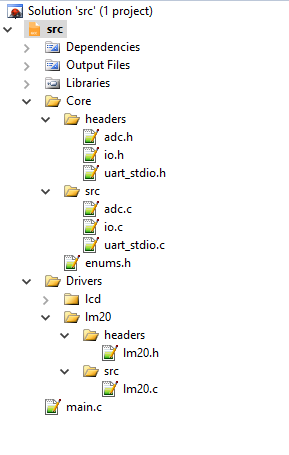
\includegraphics[width=0.6\textwidth]{solution/images/src.png}
}


%----------------------------------------------------------------------------------------
%	MAIN PROGRAM SUBSECTION
%----------------------------------------------------------------------------------------

\subsection{Main program flow}
\begin{enumerate}
	\item Global variable declarations.
	\item button1 connection
    \item button2 connection
    \item lm20 init
    \item LCD init
    \item uart init
	\item Start infinite loop (Controller life cycle)
    \begin{enumerate}
		\item get temperature from lm20
        \item if button1 pressed then display kelvin
        \item if button2 pressed then display celsius
	\end{enumerate}
\end{enumerate}

%----------------------------------------------------------------------------------------
%	PROTEUS SUBSECTION
%----------------------------------------------------------------------------------------

\newpage
\subsection{Circuit in Proteus}
I've connected MCU to Virtual Terminal. Because I use only data transmission on one direction (OUTPUT) we need to make sure that our MC Tx is connected to Peripheral Rx. Also I connected LM20 to ADC pin 3 and also connected LCD.\\\\
\centerline{
	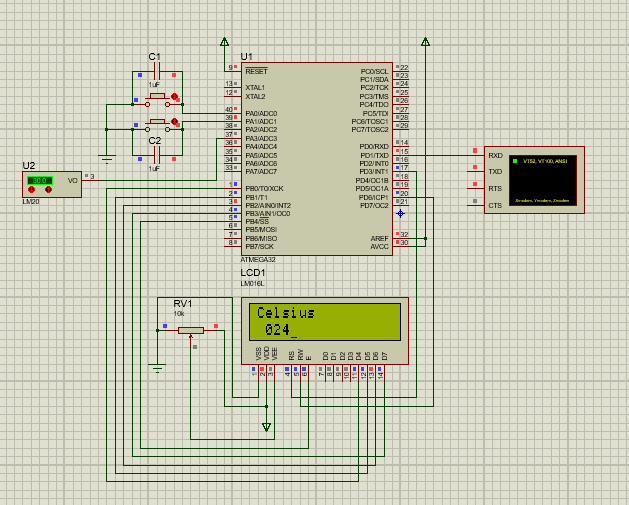
\includegraphics[width=1.0\textwidth]{solution/images/schematics.png}
}

%----------------------------------------------------------------------------------------
%	SIMULATION SUBSECTION
%----------------------------------------------------------------------------------------
\subsection{Simulation}
\centerline{
	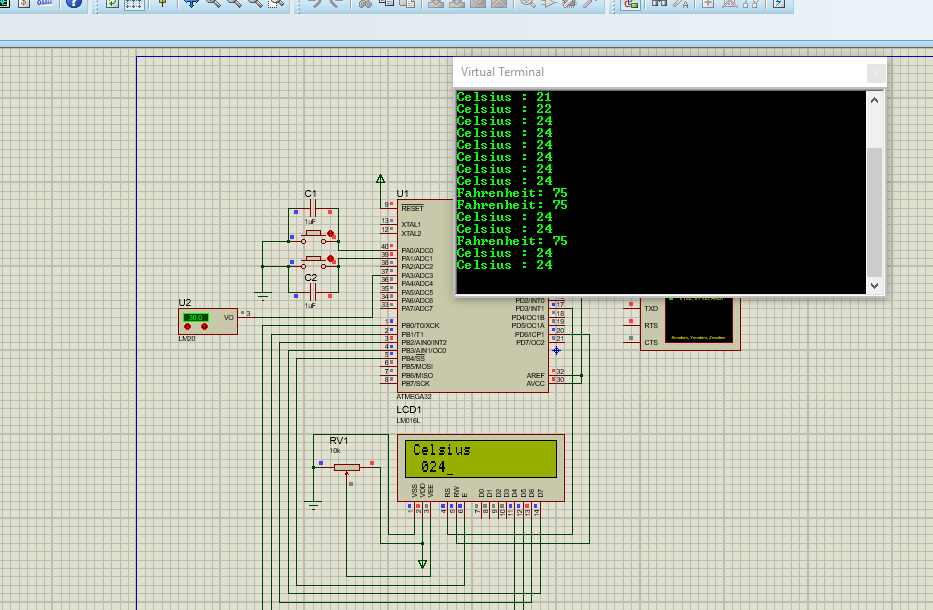
\includegraphics[width=1.0\textwidth]{solution/images/result.png}
}

